\documentclass[handout]{beamer}

\usepackage[T2A]{fontenc}			% кодировка
\usepackage[utf8]{inputenc}			% кодировка исходного текста
\usepackage[english,russian]{babel}
\usepackage{tikz}

\usepackage[first=1, last=18]{lcg}
\newcommand{\random}{\rand\arabic{rand}}

\setbeamertemplate{background canvas}[vertical shading [bottom=blue!10,top=blue!10]
\usetheme{CambridgeUS}
\usecolortheme{dove}

\setbeamercovered{dynamic}
\title{Решение задачи про робота и монетки}
\subtitle{с помощью динамики}
\author{Даниэль Ползик}
\date{\today}

\begin{document}

\begin{frame}

\titlepage

\end{frame}

\begin{frame}
  \transdissolve[duration=0.2]
  \frametitle{Условие}

\begin{block}{}
Робот Павел стоит в нижнем левом углу прямоугольного поля $n\times m$. В каждой клетке прямоугольника лежат монеты. Павел умеет ходит по клеткам вверх, вправо и по диагоналям. Ему нужно дойти до верхнего правого угла, собрав по пути как можно больше монет. Помогите Павлу разбогатеть.
Посчитайте наибольшее количесво монет, которое Павел может собрать и постройте этот маршрут. 

\end{block}

\begin{tikzpicture}[xscale=2.0, yscale=2.0]
\draw (-1.4, 0);
\foreach \x in {0,0.5,...,3}
\foreach \y in {0,0.5,...,1.5}
{
\draw (\x, \y) rectangle ++(0.5, 0.5);
\node at (\x +.25, \y +.25) {\LARGE \random};
}
\fill[color = white] (0.05, 0.05) rectangle ++(.4, .4);
\node at (0.25, 0.25) {
\includegraphics[scale = 0.0225]{robot.png}};
\fill[color = white] (3.05, 1.55) rectangle ++(.4, .4);
\node at (3.25, 1.75) {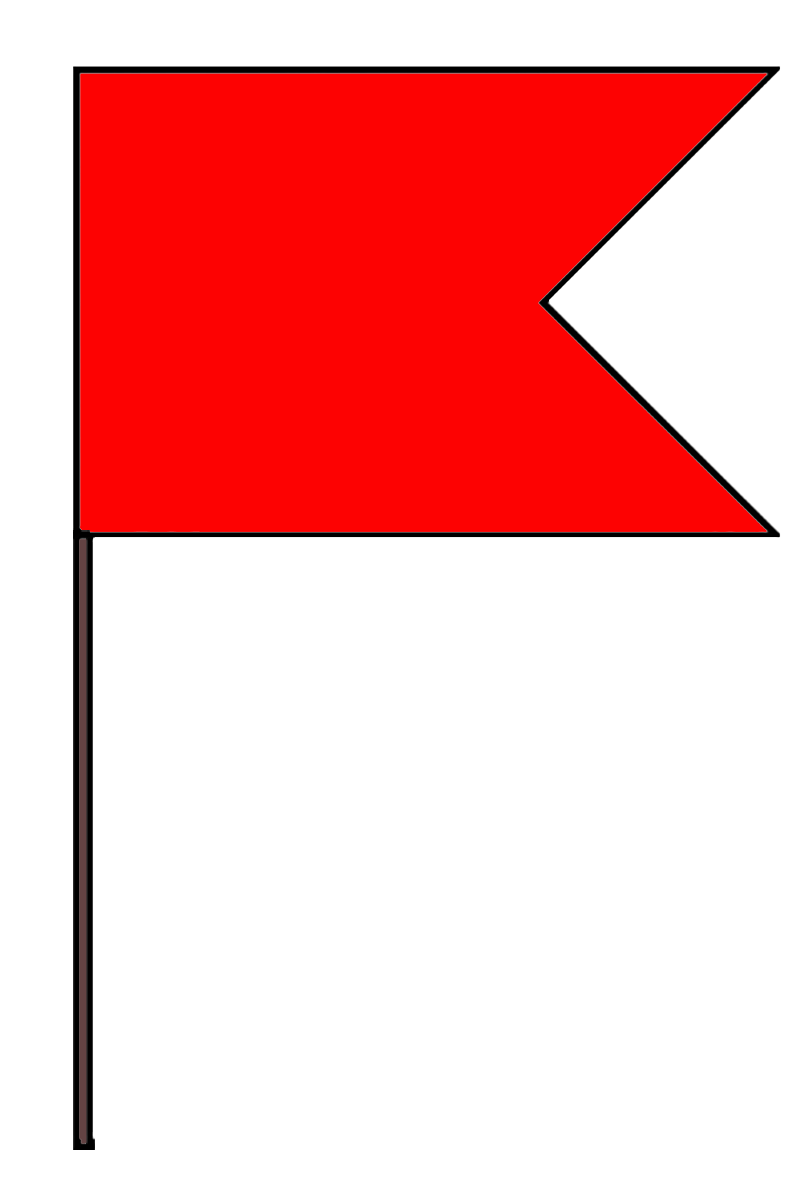
\includegraphics[scale = 0.04]{flag.png}};

\end{tikzpicture}

\end{frame}

\begin{frame}
\transdissolve[duration=0.2]
\frametitle{Идеи}
\begin{block}{}
Создадим двумерный массив $D [n \times m]$\\
В $D[i][j]$ будет храниться наибольшее количество монет, которое можно в эту клетку принести.
\end{block}
\begin{block}{}
Тогда ответом на эту задачу будет $D[n-1][m-1]$. Как раз наибольшее количество монет, которое можно туда донести.
\end{block}
\begin{block}{}
По такому массиву будет легко востановить путь с конца.
Если мы находимся в какой-то клетке $[i][j]$, то можем посмореть на те клетки, из которых мы могли прийти ($[i-1][j]$, $[i][j-1]$, $[i-1][j-1]$). Та клетка, из которой мы могли принести больше монет, нам выгоднее. Значит мы пришли из клетки в которой значение $D$ - максимально.\\
$max(D[i-1][j]$, $D[i][j-1]$, $D[i-1][j])$.
\end{block}

\end{frame}

\begin{frame}

\transdissolve[duration=0.2]
\frametitle{Заполнение массива $D$}

\begin{block}{}
Заметим, что $D[i][j] = $
$\begin{cases}
D[i-1][j] + arr[i][j];\\
D[i][j-1] + arr[i][j];\\
D[i-1][j-1] + arr[i][j]\\
\end{cases}$\\
Так как нам нужно как можно больше монет, то выберем из этих вариантов самый выгодный. То есть максимум.
\end{block}

\begin{block}{}
Если пробегать массив $D$ слева направо и преходя в конуце строки в начало следующей, записывая в:\\
$D[i][j] = max $
$\begin{cases}
D[i-1][j] + arr[i][j];\\
D[i][j-1] + arr[i][j];\\
D[i-1][j-1] + arr[i][j]\\
\end{cases}$\\
, то мы заполним массив правильно. Так как, когда мы будет заполнять $D[i][j]$, то и $D[i-1]$, и $D[i][j-1]$, и $D[i-1][j-1]$ будут уже заполнены
\end{block}
\end{frame}

\begin{frame}

\transdissolve[duration=0.2]
\frametitle{Заполнение массива $D$}

\begin{block}{Замечания}
1) $D[0][0] = 0$, так как мы оттуда начинаем и туда ничего не принести\\
2) $D[i][0] = arr[i][0] + D[i-1][0]$, так как больше нет клеток, из которых Павел мог прийти\\
3) Аналогично, $D[0][j] = arr[0][j] + D[0][j-1]$
\end{block}

\begin{block}{Пример массива D}
\begin{tikzpicture}[xscale=1.5, yscale=1.5]
\foreach \x in {0,0.5,...,3}
\foreach \y in {0,0.5,...,1.5}
{
\draw (\x, \y) rectangle ++(0.5, 0.5);
}
\node at (0.25, 0.25) {
\includegraphics[scale = 0.0175]{robot.png}};
\draw[ultra thick, ->, blue] (0.4,0.25) -- (0.6,0.25);
\node at (0.75, 0.25) {\LARGE 2};
\draw[ultra thick, ->, blue] (0.75,0.4) -- (0.75,0.6);
\node at (1.25, 0.25) {\LARGE 3};
\node at (1.75, 0.25) {\LARGE 0};
\node at (2.25, 0.25) {\LARGE 3};
\node at (2.75, 0.25) {\LARGE 3};
\node at (3.25, 0.25) {\LARGE 12};

\node at (0.25, 0.75) {\LARGE 1};
\node at (0.75, 0.75) {\LARGE 4};
\draw[ultra thick, ->, blue] (0.9,0.75) -- (1.1,0.75);
\node at (1.25, 0.75) {\LARGE 2};
\draw[ultra thick, ->, blue] (1.4,0.75) -- (1.6,0.75);
\node at (1.75, 0.75) {\LARGE 9};
\draw[ultra thick, ->, blue] (1.9,0.75) -- (2.1,0.75);
\node at (2.25, 0.75) {\LARGE 7};
\draw[ultra thick, ->, blue] (2.4,0.75) -- (2.6,0.75);
\node at (2.75, 0.75) {\LARGE 3};
\draw[ultra thick, ->, blue] (2.75,0.9) -- (2.75,1.1);
\node at (3.25, 0.75) {\LARGE 2};

\node at (0.25, 1.25) {\LARGE 1};
\node at (0.75, 1.25) {\LARGE 1};
\node at (1.25, 1.25) {\LARGE 8};
\node at (1.75, 1.25) {\LARGE 5};
\node at (2.25, 1.25) {\LARGE 1};
\node at (2.75, 1.25) {\LARGE 5};
\draw[ultra thick, ->, blue] (2.9,1.25) -- (3.1,1.25);
\node at (3.25, 1.25) {\LARGE 3};
\draw[ultra thick, ->, blue] (3.25,1.4) -- (3.25,1.6);


\node at (0.25, 1.75) {\LARGE 5};
\node at (0.75, 1.75) {\LARGE 3};
\node at (1.25, 1.75) {\LARGE 2};
\node at (1.75, 1.75) {\LARGE 2};
\node at (2.25, 1.75) {\LARGE 6};
\node at (2.75, 1.75) {\LARGE 2};
\node at (3.25, 1.75) {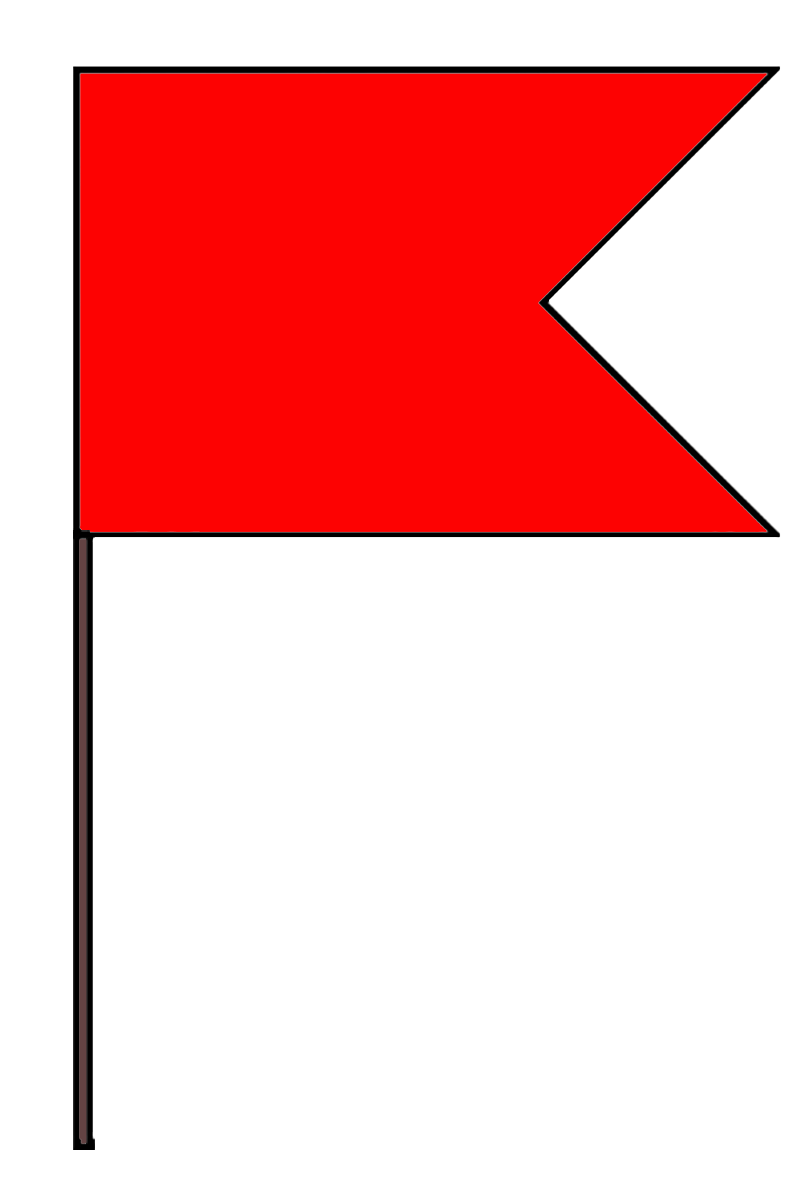
\includegraphics[scale = 0.03]{flag.png}};

\foreach \x in {4,4.5,...,7}
\foreach \y in {0,0.5,...,1.5}
{
\draw (\x, \y) rectangle ++(0.5, 0.5);
}

\node at (4.25, 0.25) {\color{blue} \LARGE 0};
\node at (4.75, 0.25) {\color{blue} \LARGE 2};
\node at (5.25, 0.25) {\LARGE 5};
\node at (5.75, 0.25) {\LARGE 5};
\node at (6.25, 0.25) {\LARGE 8};
\node at (6.75, 0.25) {\LARGE 11};
\node at (7.25, 0.25) {\LARGE 23};

\node at (4.25, 0.75) {\LARGE 1};
\node at (4.75, 0.75) {\color{blue} \LARGE 6};
\node at (5.25, 0.75) {\color{blue} \LARGE 8};
\node at (5.75, 0.75) {\color{blue} \LARGE 17};
\node at (6.25, 0.75) {\color{blue} \LARGE 24};
\node at (6.75, 0.75) {\color{blue} \LARGE 27};
\node at (7.25, 0.75) {\LARGE 29};

\node at (4.25, 1.25) {\LARGE 2};
\node at (4.75, 1.25) {\LARGE 7};
\node at (5.25, 1.25) {\LARGE 16};
\node at (5.75, 1.25) {\LARGE 22};
\node at (6.25, 1.25) {\LARGE 25};
\node at (6.75, 1.25) {\color{blue} \LARGE 32};
\node at (7.25, 1.25) {\color{blue} \LARGE 35};

\node at (4.25, 1.75) {\LARGE 7};
\node at (4.75, 1.75) {\LARGE 10};
\node at (5.25, 1.75) {\LARGE 18};
\node at (5.75, 1.75) {\LARGE 24};
\node at (6.25, 1.75) {\LARGE 31};
\node at (6.75, 1.75) {\LARGE 34};
\node at (7.25, 1.75) {\color{blue} \LARGE 35};

\end{tikzpicture}


\end{block}

\end{frame}

\end{document}
